\documentclass[main]{subfiles}

\begin{document}
    \Date{10.09.19}
    \subsection{Задачи на кривые}

    Мы хотим найти $\tau$ через $\dot{\gamma},\ \ddot{\gamma},\ \dddot{\gamma}$
    \begin{remark}
      На плоскоти в каждой точке гладкой кривой есть окружность, которая наилучшим образом приближает кривую
      \[R=\frac{1}{|\ddot{\gamma}|},\q |\ddot{\gamma}| := \ae \text{ - кривизна}\]
      \begin{figure}[h]
          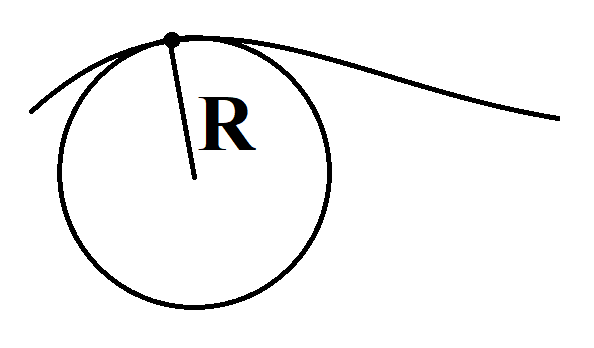
\includegraphics[scale=0.3]{pics/2_1.png}
          \centering
      \end{figure}
    \end{remark}
    \begin{Sol} [продолжение]
      \[\tau = <\frac{d N}{dt},\ B>\]
      \[\frac{d N}{dt} = \Br{\frac{\ddot{\gamma}}{\abs{\ddot{\gamma}}}}' = \frac{\dddot{\gamma} |\ddot{\gamma}| - |\ddot{\gamma}|' \ddot{\gamma}}{|\ddot{\gamma}|^2}\]
      \begin{multline*}
        \Ra <\frac{d N}{dt},\ B>=<\frac{\dddot{\gamma} |\ddot{\gamma}| - |\ddot{\gamma}|' \ddot{\gamma}}{|\ddot{\gamma}|^2},\ \frac{\dot{\gamma} \times \ddot{\gamma}}{|\ddot{\gamma}|}> = \\
        \qq \qq = \frac{1}{|\ddot{\gamma}|^3} <\dddot{\gamma} |\ddot{\gamma}|-|\ddot{\gamma}|' \ddot{\gamma},\ \dot{\gamma} \times \ddot{\gamma}> \us{\text{см. на N}}{=} \\
        = \frac{1}{|\ddot{\gamma}|^3} <\dddot{\gamma} |\ddot{\gamma}|,\ \dot{\gamma} \times \ddot{\gamma}> = \frac{1}{|\ddot{\gamma}|^2} <\dddot{\gamma},\ \dot{\gamma} \times \ddot{\gamma} > = \frac{(\dot{\gamma},\ \ddot{\gamma},\ \dddot{\gamma})}{|\ddot{\gamma}|^2}
      \end{multline*}
    \end{Sol}

    \begin{Example}
      \[\gamma: \R \ra \R^3,\q t \mapsto (4 \cos(t),\ 5-5 \sin(t),\ -3\cos(t))\]
      \begin{enumerate}
        \item Найти $\ae$ и $\tau$
        \item Понять, что из себя представляет линия
      \end{enumerate}
    \end{Example}

    \begin{sol}
      \begin{enumerate}
        \item Предыдущую задачу мы не можем просто так применить, потому что $|\dot{\gamma}|=5 \neq 1$, но мы можем перепараметризовать:
        \[\w{\gamma}: \R \ra \R^3,\q t \mapsto (4 \cos(\frac{t}{5}),\ 5-5 \sin(\frac{t}{5}),\ -3\cos(\frac{t}{5}))\]
        \[\w{\dot{\gamma}} = (-\frac{4}{5} \sin(\frac{t}{5}),\ -\cos(\frac{t}{5}),\ \frac{3}{5} \sin(\frac{t}{5}))\]
        \[\Ra |\w{\dot{\gamma}}|=1\]
        \[\w{\ddot{\gamma}} = (-\frac{4}{25} \cos(\frac{t}{5}),\ \frac{1}{5} \sin(\frac{t}{5}),\ \frac{3}{25} \cos(\frac{t}{5}))\]
        \[\Ra \ae = |\w{\ddot{\gamma}}| = \frac{1}{25}\]
        \[\w{\dddot{\gamma}} = (\frac{4}{125} \sin(\frac{t}{5}),\ \frac{1}{25} \cos(\frac{t}{5}),\ -\frac{3}{125} \sin(\frac{t}{5}))\]
        \[\Ra \tau = \frac{(\dot{\gamma},\ \ddot{\gamma},\ \dddot{\gamma})}{|\ddot{\gamma}|^2}=25 (\dot{\gamma},\ \ddot{\gamma},\ \dddot{\gamma})=0\]
        \item Наша линия находится на плоскости:
        \[3x+0y+4z\]
        И лежит на сфере:
        \[x^2+(y-5)^2+z^2=25\]
        Значит она представляет из себя окружность, потому что есть разные точки
        \begin{figure}[H]
            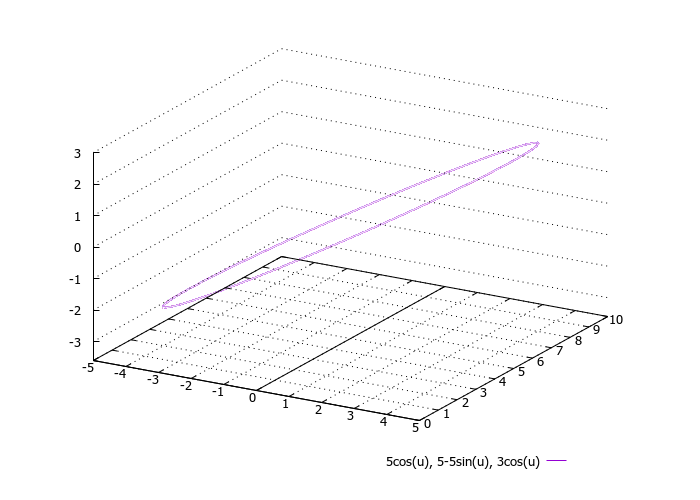
\includegraphics[scale=0.6]{pics/2_2.png}
            \centering
        \end{figure}
      \end{enumerate}
    \end{sol}

    \begin{Example}
      \[\gamma: \R \ra \R^3,\q t \mapsto (\cos(t),\ \sin(t),\ t)\]
      \begin{enumerate}
        \item Построить график
        \begin{figure}[H]
            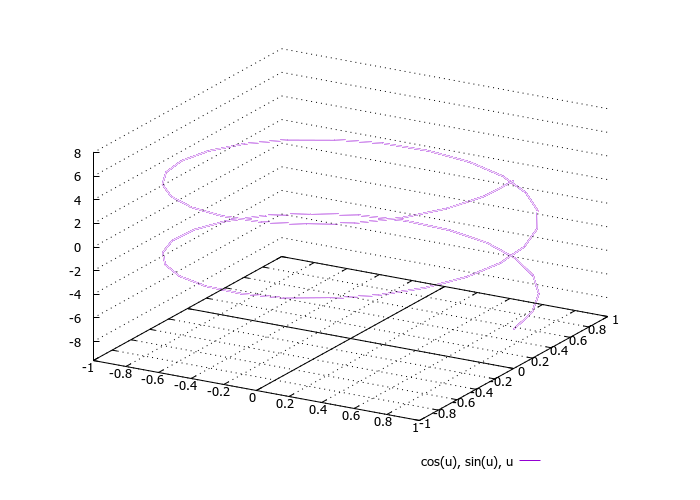
\includegraphics[scale=0.6]{pics/2_3.png}
            \centering
        \end{figure}
        \item Найти $\ae$ и $\tau$
      \end{enumerate}
    \end{Example}

    \begin{sol}
        Аналогично $t \ra \dfrac{t}{\sqrt{2}}$
        \[\w{\gamma}: \R \ra \R^3,\q t \mapsto (\cos(\frac{t}{\sqrt{2}}),\ \sin(\frac{t}{\sqrt{2}}),\ \frac{t}{\sqrt{2}})\]
        \[\w{\dot{\gamma}}=(-\frac{1}{\sqrt{2}} \sin(\frac{t}{\sqrt{2}}),\ \frac{1}{\sqrt{2}} \cos(\frac{t}{\sqrt{2}}),\ \frac{1}{\sqrt{2}})\]
        \[\Ra |\w{\dot{\gamma}}|=1\]
        \[\w{\ddot{\gamma}}=(-\frac{1}{2} \cos(\frac{t}{\sqrt{2}}),\ -\frac{1}{2} \sin(\frac{t}{\sqrt{2}}),\ 0)\]
        \[\Ra \ae = |\w{\ddot{\gamma}}| = \frac{1}{2}\]
        \[\w{\dddot{\gamma}}=(\frac{1}{2 \sqrt{2}} \sin(\frac{t}{\sqrt{2}}),\ -\frac{1}{2 \sqrt{2}} \cos(\frac{t}{\sqrt{2}}),\ 0)\]
        \[\tau = \frac{(\dot{\gamma},\ \ddot{\gamma},\ \dddot{\gamma})}{|\ddot{\gamma}|^2}\]
        \[(\dot{\gamma},\ \ddot{\gamma},\ \dddot{\gamma}) = \det
        \begin{pmatrix}
          -\frac{1}{\sqrt{2}} \sin(\frac{t}{\sqrt{2}}) & \frac{1}{\sqrt{2}} \cos(\frac{t}{\sqrt{2}}) & \frac{1}{\sqrt{2}}\\ \\
          -\frac{1}{2} \cos(\frac{t}{\sqrt{2}}) & -\frac{1}{2} \sin(\frac{t}{\sqrt{2}}) & 0\\ \\
          \frac{1}{2 \sqrt{2}} \sin(\frac{t}{\sqrt{2}}) & -\frac{1}{2 \sqrt{2}} \cos(\frac{t}{\sqrt{2}}) & 0
        \end{pmatrix} = \frac{1}{8}\]
    \end{sol}
\end{document}
